\section{Stato dell'arte dei moduli PPG}
Di seguito vengono presentati alcuni moduli attualmente in commercio per l'acquisizione di segnali fotopletismografici, che si differenziano per caratteristiche e prestazioni. Si è cercato di mettere in evidenza le peculiarità di ogni modulo che giustificano il loro utilizzo in diverse situazioni. Sono proposti tre moduli prodotti dalla Maxim Integrated e un sensore di Analog Devices.

\textbf{MAX86916} Il modulo MAX86916 è un sensore ottico integrato per applicazioni di bio-sensing e prossimità prodotto da Maxim Integrated\cite{IntegratedMAX86916}. Include quattro LED (rosso, infrarosso, verde, blu), un fotodiodo, elementi ottici e elettronica a basso rumore per circuiti di rimozione della luce ambientale. Il sensore è progettato per agevolare l'utilizzo in dispositivi indossabili, smartphone e assistenti per il fitness. Infatti presenta dimensioni molto ridotte (3.5 mm x 7.0 mm x 1.5 mm) e bassi consumi. Il modulo utilizza una singola alimentazione da 1.8 V e un'alimentazione separata di 5.5 V per i LED interni. \`E possibile comunicare con il modulo attraverso un'interfaccia standard I\ap{2}C. Spesso è utilizzato per misurazioni di frequenza cardiaca e saturazione di ossigeno in piattaforme di sensori bio-ottici in modalità riflessiva. Presenta un ADC a 19 bit con frequenza di campionamento programmabile da 50 Hz a 3200 Hz. Il dispositivo integra anche una funzione di prossimità che permette di ridurre la luce visibile e i consumi quando non rileva una superficie vicina. Inoltre, grazie alla presenza di un \textit{Ambient Light Cancellation} (ALC) e di un \textit{Cross Talk Cancellation} è possibile ridurre gli errori di misura causati dall'interferenza della luce ambientale e degli elementi ottici usati. Possiede anche un buffer FIFO che permette di salvare i dati acquisiti senza la necessità di una lettura continua di un microcontrollore.
\begin{figure}[h]
	\centering
	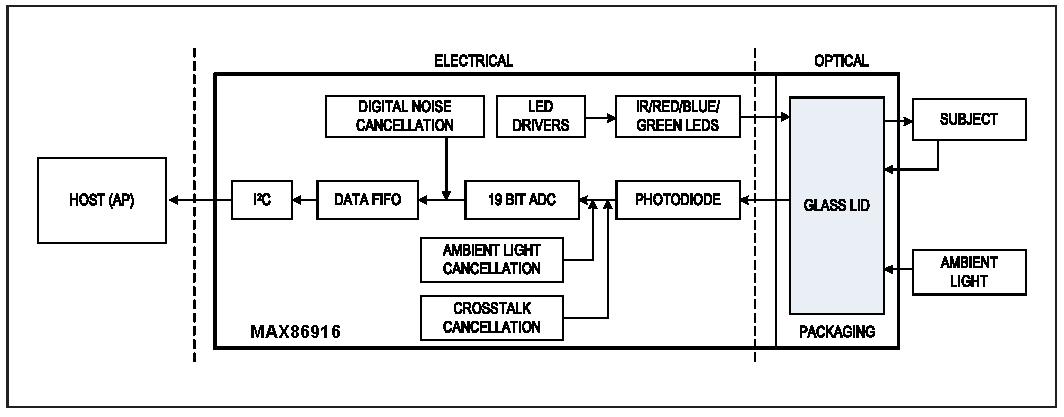
\includegraphics[width=1\linewidth]{ImageFiles/Fotopletismografia/MAX86916BlockDiagram}
	\caption{Schema a blocchi del modulo MAX86916.}
	\label{fig:MAX86916BlockDiagram}
\end{figure}

\textbf{MAXM86161} Il MAXM86161 è un sistema di acquisizione di dati ottici completamente integrato a basso consumo prodotto da Maxim Integrated\cite{IntegratedMAXM86161}. All'interno sono presenti tre LED (rosso, infrarosso e verde) e un fotodiodo PIN ad alta efficienza. Grazie alle sue dimensioni ridotte (2.9 mm x 4.3 mm x 1.4 mm) è possibile utilizzarlo in dispositivi indossabili ed è ottimizzato per applicazioni intra-auricolari. \`E ideale per misure ottiche di battito cardiaco, SpO\ped{2} e monitoraggio continuo per HRV (Heart Rate Variability) con tecnologia riflessiva. Il sensore opera con una singola tensione di alimentazione che deve essere compresa tra i 3.0V a 5.5V. Essa permette l'alimentazione sia dei LED sia dell'elettronica interna, grazie a un LDO integrato che genera una tensione in uscita di 1.8V. Ogni dispositivo contiene un buffer FIFO a 128 word e presenta un ADC a 19-bit. Per eliminare interferenze con la luce esterna, il sensore integra un circuito di cancellazione della luce ambientale e un'algoritmo di rilevamento e sostituzione chiamato \textit{picket fence}. Infatti, in alcune situazioni in cui la luce ambientale varia molto rapidamente (per esempio quando si è in macchina o esposti alla luce solare) l'ALC potrebbe produrre una stima errata della luce ambientale. In queste condizioni estreme, la misurazione viene corretta grazie alla funzione \textit{picket fence}. In aggiunta, è disponibile una funzione di prossimità che permette di ridurre significativamente il consumo di energia quando il modulo non è a contatto con la pelle in modo da aumentare la durata della batteria nei dispositivi portatili. 
\begin{figure}[h]
	\centering
	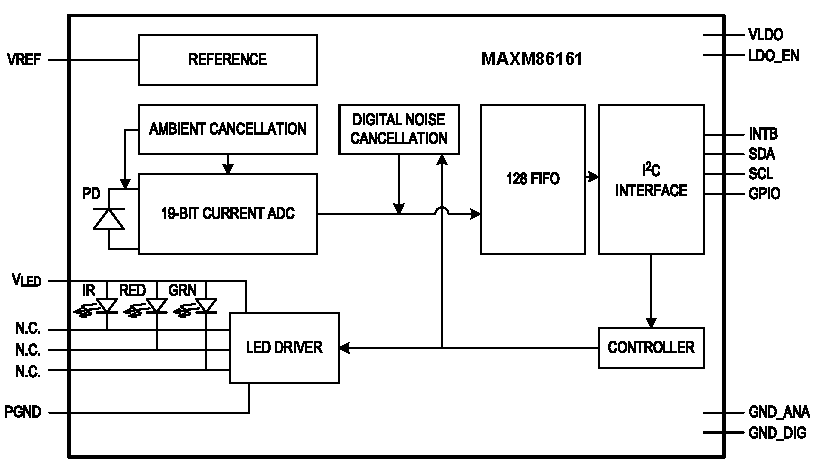
\includegraphics[width=0.7\linewidth]{ImageFiles/Fotopletismografia/MAXM86161BlockDiagram}
	\caption{Schema a blocchi del modulo MAXM86161.}
	\label{fig:MAXM86161BlockDiagram}
\end{figure}

\textbf{MAX30101} Il sensore MAX30101 è un modulo integrato che permette di effettuare acquisizioni fotopletismografiche per misurazioni di ossimetria e di frequenza cardiaca prodotto da Maxim Integrated\cite{IntegratedMAX30101}. Esso fornisce un sistema completo progettato per essere facilmente integrato in dispositivi portatili e indossabili. Presenta dimensioni ridotte (5.6 mm x 3.3 mm x 1.55 mm) integrando tre LED (rosso, infrarosso e verde), un fotodiodo, elementi ottici e elettronica a basso rumore. Il modulo richiede due alimentazioni: una singola alimentazione di 1.8V, per alimentare i circuiti interni, e una di 5.0V, per alimentare i LED integrati. Presenta un'interfaccia I\ap{2}C per la lettura e la scrittura dei registri interni. \`E presente anche un buffer FIFO che permette al microcontrollore collegato la lettura discontinua dei dati acquisiti. All'interno del modulo è presente anche un sensore di temperatura le cui misure sono utilizzate da un algoritmo interno per migliorare la stima del grado di ossigenazione. Quando viene attivata una delle due modalità permesse (HR o SpO\ped{2}), viene anche inizializzata la funzione di prossimità che permette di ridurre i consumi.   
\begin{figure}[tb]
	\centering
	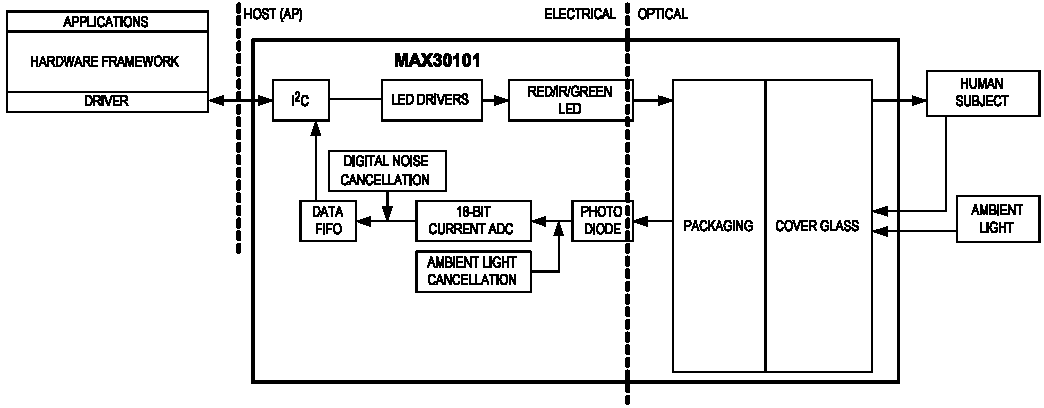
\includegraphics[width=1\linewidth]{ImageFiles/Fotopletismografia/MAX30101BlockDiagram}
	\caption{Schema a blocchi del modulo MAX30101.}
	\label{fig:MAX30101BlockDiagram}
\end{figure}

\pagebreak

\textbf{ADPD144RI} Il modulo ADPD144RI è un sensore elettro-ottico ottimizzato per la misure fotopletismografiche dell'ossigenazione del sangue proposto da Analog Devices\cite{AnalogDevicesADPD144RI}. Grazie a rilevazioni sincrone nelle regioni del rosso e infrarosso è possibile ottenere misurazioni di alta qualità, permettendo l'eliminazione delle componenti DC e AC della luce ambientale, mantenendo un basso consumo di potenza. Integra un LED rosso (660 nm) e un LED infrarosso (880 nm) come sorgenti luminose e un fotodiodo a 4 canali per l'acquisizione. Inoltre, il package è stato pensato per fornire un isolamento ottico tra i led e i fotodiodi in modo da migliorare il rapporto segnale rumore (SNR), garantendo che la luce attraversi i tessuti prima di essere acquisita. Il dispositivo viene alimentato con una tensione di 1.8V per i circuiti interni e una tensione di 3.5V per l'alimentazione dei LED. Le dimensioni del package sono 2.8 mm x 5.0 mm x 1.35 mm e presenta un'interfaccia I\ap{2}C per la lettura diretta dei registri oppure del buffer FIFO. \`E possibile anche collegare fino a due LED esterni per realizzare misurazioni PPG con tecnologia trasmissiva.
\begin{figure}[b]
	\centering
	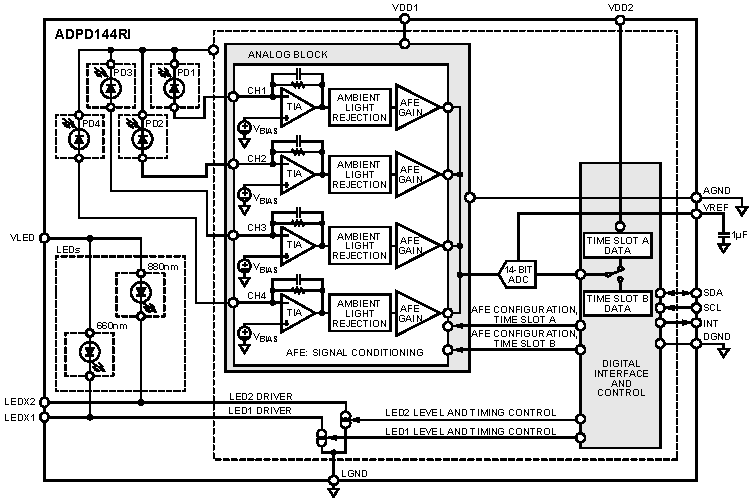
\includegraphics[width=0.8\linewidth]{ImageFiles/Fotopletismografia/ADPD144RIBlockDiagram}
	\caption{Diagramma funzionale del modulo ADPD144RI.}
	\label{fig:ADPD144RIBlockDiagram}
\end{figure}
\clearpage
\noindent Nella tabella \ref{tab:ModuliPPG} vengono riassunte le caratteristiche dei moduli sopra presentati.
\begin{table}[h]
	\renewcommand{\arraystretch}{1.5}
	\centering
	\begin{tabular}{ccccc}
		\hline
		& MAX86916    & MAXM86161   & MAX30101  & ADPD144RI    \\ \hline
		Lunghezza {[}mm{]}     & 3.5         & 2.9         & 5.6       & 2.8          \\ \hline
		Larghezza {[}mm{]}     & 7.0         & 4.3         & 3.3       & 5.0          \\ \hline
		Altezza {[}mm{]}       & 1.5         & 1.4         & 1.55      & 1.35         \\ \hline
		V\ped{DD} {[}V{]}          & 1.7 - 2.0   & /           & 1.7 - 2.0 & 1.7 - 1.9    \\ \hline
		V\ped{LED} {[}V{]}         & 3.5 - 5.5   & 3.0 - 5.5   & 3.1 - 5.0 & 3 - 4.3      \\ \hline
		V\ped{LDO} {[}V{]}         & /           & 1.68 - 1.92 & /         & /            \\ \hline
		Interfaccia            & I\ap{2}C       & I\ap{2}C       & I\ap{2}C     & I\ap{2}C        \\ \hline
		\textit{f\ped{s}} {[}Hz{]}          & 50 - 3200   & 8 - 4096    & 50 - 3200 & 0.122 - 3480 \\ \hline
		Risoluzione {[}bit{]}  & 19          & 19          & 19        & 14           \\ \hline
		Led integrati          & R, IR, G, B & R, IR, G    & R, IR, G  & R, IR        \\ \hline
		\# fotodiodi integrati & 1           & 1           & 1         & 4            \\ \hline
	\end{tabular}
	\caption{Riepilogo delle caratteristiche dei moduli PPG.}
	\label{tab:ModuliPPG}
\end{table}
\todo{Inserire altro materiale? Dispositivi, algoritmi...}